 \section{Uvod i definicija}

Kombinatorne igre vrsta su igara u kojima se igrači bore za kontrolu nad skupom objekata, poput figura na šahovnici ili polja na ploči. Ove igre zovu se kombinatorne jer se igrači bore za kontrolu nad kombinacijom objekata i svojom strategijom igrači koriste svoje znanje i vještinu za kontrolu igre i ukupnu pobjedu.\newline

Za svaku kombinatornu igru vrijede sljedeći uvjeti\cite{garner2007combinatorialgametheory}:

\begin{itemize}
    \item Dva igrača: Kombinatorne igre igraju se između dva igrača, koji mogu biti označeni različitim bojama, znakovima ili samo kao prvi i drugi igrač. 
    \item Nema elemenata slučajnosti: U kombinatornim igrama, nema faktora slučajnosti koji bi utjecali na ishod igre. To znači da potezi koje igrači čine nisu određeni kockanjem, srećom ili nasumičnim događajima, već samo njihovom strategijom.
    \item Potpuna informacija: Svaki igrač u kombinatornoj igri ima potpuni uvid u sve informacije o trenutnom stanju igre. Nema skrivanja idućeg poteza, svaki igrač zna sve što je javno dostupno.
    \item Naizmjenična igra: Kombinatorne igre igraju se naizmjenično između dva igrača. Svaki igrač izvodi poteze jedan za drugim, izmjenjujući se dok igra ne završi.
    \item Postoji pobjednik: U kombinatornim igrama, jedan igrač uvijek mora pobijediti, a drugi izgubiti. Nema neodlučenog rezultata kao što je remi u šahu.
    \item Uvjet pobjede: Da bi igrač pobijedio, potrebno je doći do krajnje pozicije igre koja je unaprijed definirana. Ova krajnja pozicija može biti, na primjer, osvajanje protivničkog kralja u šahu ili postizanje zadane razine bodova u igri kao što je Go. 
\end{itemize}


Također, moramo uvesti još jedan pojam, a to je nepristrana igra\cite{2001winningwaysforyourmathematicalplays}.

\begin{definition}
Igra je nepristrana ako i samo ako oba igrača imaju iste mogućnosti poteza za svaku trenutnu poziciju u igri.
\end{definition}
 


U svim nepristranim kombinatornim igrama postoje dvije vrste pozicija: \textit{P-pozicije} (engl. previous) i \textit{N-pozicije} (engl. next). P-pozicije su pozicije u kojima prethodni igrač ima pobjedničku strategiju, a sukladno tome, N-pozicije su pozicije u kojima sljedeći igrač ima pobjedničku strategiju. Postupak za određivanje vrste pozicije kojoj pripada određena pozicija započinje identificiranjem završnih, terminalnih pozicija kao P-pozicija. Zatim se identificiraju pozicije koje vode do P-pozicija i označavaju se kao N-pozicije. Nakon toga, traže se pozicije iz kojih se dolazi samo do N-pozicija i takve pozicije se označavaju kao P-pozicije, a to se sve ponavlja dok se ne odrede i identificiraju sve moguće pozicije u igri kao P-pozicije ili N-pozicije.

Ova podjela na P-pozicije i N-pozicije korisna je pri razvoju pobjedničke strategije u igri jer je cilj svakog igrača dovesti igru u P-pozicije, a to su pobjedničke pozicije. Također, početna pozicija određuje koji igrač ima pobjedničku strategiju. U idućem poglavlju analizirat ćemo P-pozicije i N-pozicije na primjerima igre 21 i igre Nim. 



\section{Primjeri kombinatornih igara}

Postoje brojne popularne kombinatorne igre, a ovdje ćemo nabrojati samo neke od njih:

\subsection*{Igra oduzimanja}

Vjerojatno najjednostavniji mogući primjer jedne nepristrane kombinatorne igre je \textit{igra oduzimanja}. U igri oduzimanja dva igrača miču jedan, dva ili tri žetona sa hrpe koja se sastoji od 21 žetona. Gubitnik je onaj igrač koji ukloni zadnji žeton. Postoji mnogo mogućih varijacija ove igre, od broja dozvoljenih žetona koji se mogu ukloniti u jednom potezu, do ukupnog broja žetona na hrpi. U nastavku analize pokazat ćemo kako varijacije utječu na rezultat igre i strategiju igrača.



\subsection*{Nim}


Igra Nim također je jedna jednostavna igra za dva igrača u kojoj se, za razliku od igre oduzimanja, koristi više hrpa žetona. Svaka hrpa žetona može imati proizvoljan broj žetona, a broj hrpa može biti različit od igre do igre. Na početku igre, igrači se dogovaraju o broju hrpa i broju žetona u svakoj hrpi.

Tijekom igre, igrači naizmjence uzimaju žetone s ploče za igru. Svaki igrač mora uzeti žetone samo iz jedne hrpe, ali može uzeti bilo koji broj žetona iz te hrpe. Nakon što igrač uzme žetone, on ih uklanja s ploče za igru.

Cilj igre je ostati s barem jednim žetonom na ploči, tako da protivnik ne može uzeti zadnji žeton. Uzimanje zadnjeg žetona predstavlja gubitak igre, a pobjednik je onaj koji uspije natjerati protivnika da uzme zadnji žeton.

\begin{figure}[H]
\centering
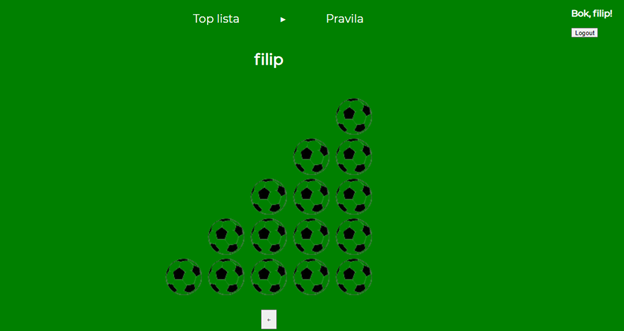
\includegraphics[width=14cm]{slike-program/Slika6.png}
\caption{Igra Nim.}
\label{}
\end{figure}


\subsection*{Hex}

Igra Hex igra je za dva igrača koja se igra na šesterokutnoj ploči koja se sastoji od šestokutnih polja. Jedan igrač igra s bijelim figurama, a drugi s crnim figurama. Igrači igraju naizmjenično, stavljajući svoje figure na polja ploče.

Cilj igre je stvoriti poveznicu između dvije suprotne strane šesterokuta koju čine igračeve figure. Bijeli igrač pokušava stvoriti poveznicu između suprotne bijele strane ploče, dok crni igrač pokušava stvoriti poveznicu između suprotne crne strane ploče. Pobjeđuje igrač koji prvi uspije stvoriti poveznicu od jedne do druge strane ploče.

Figure se mogu postavljati na bilo koje slobodno polje na ploči. Igrači nastoje blokirati protivnika i povezati svoje figure kako bi stvorili poveznicu. Igrači također pokušavaju onemogućiti stvaranje poveznice za protivnika.


\subsection*{Go}

Igra Go igra je za dva igrača koja se igra na ploči veličine 19x19 polja, ali može se igrati i na manjim pločama. Jedan igrač igra crnim figurama, dok drugi igrač igra bijelim figurama. Igrači igraju naizmjenično, stavljajući svoje figure na prazna polja ploče.

Cilj igre je osvojiti što više teritorija na ploči postavljanjem svojih figura na prazna polja i stvaranjem zatvorenih prostora oko tih figura. Figura se naziva kamenom, a igrači ih postavljaju na presjecišta linija koje čine ploču.

Kamenovi se mogu postavljati na bilo koje prazno polje, ali ne smiju se postavljati na polja koja su već okupirana od strane protivnika. Kada jedan igrač okruži prazna polja kamenovima, taj teritorij smatra se osvojenim.

Osim osvajanja teritorija, igrači također mogu zarobiti protivničke kamenove. Kamen se zarobi kada se okruži na sve strane praznim poljima ili poljima s kamenovima iste boje. Zarobljeni kamen se uklanja s ploče.

Igra Go je za razliku od ostalih navedenih igara vrlo složena i strateški izazovna igra u kojoj  igrači pokušavaju predvidjeti poteze protivnika i stvoriti najbolju strategiju za osvajanje teritorija.
